\documentclass{article}
\usepackage[utf8]{inputenc}
\usepackage[margin=0.8in]{geometry}
\usepackage{amsmath}
\usepackage{graphicx}
\usepackage{amsthm}
\usepackage{algorithm}
\usepackage{algpseudocode}
\usepackage{enumitem}
\usepackage{verbatim}
\usepackage{tikz-qtree}
\usepackage{color, soul}
\usepackage{makecell}
% \usepackage{qtree}
\graphicspath{ {./} }

\title{CS190I HW3 Report}
\author{Matthew Ho}
\date{February 2022}

\usepackage{listings}
\usepackage{color}

\definecolor{codegreen}{rgb}{0,0.6,0}
\definecolor{codegray}{rgb}{0.5,0.5,0.5}
\definecolor{codepurple}{rgb}{0.58,0,0.82}
\definecolor{backcolour}{rgb}{0.95,0.95,0.92}

\lstdefinestyle{style1}{
}

\algnewcommand{\var}{\texttt}

\lstset{
    commentstyle=\color{codegreen},
    keywordstyle=\color{magenta},
    numberstyle=\tiny\color{codegray},
    stringstyle=\color{codepurple},
    basicstyle=\ttfamily\footnotesize,
    breakatwhitespace=false,         
    breaklines=true,                 
    captionpos=b,                    
    keepspaces=true,                 
    numbers=left,                    
    numbersep=2pt,                  
    showspaces=false,                
    showstringspaces=false,
    showtabs=false,                  
	xleftmargin=5.0ex,
    tabsize=2,
	breaklines=true,
    postbreak=\mbox{\textcolor{red}{$\hookrightarrow$}\space}
}


\begin{document}
\maketitle

\section{Collaboration}
Did you receive any help whatsover from anyone in solving this assignment? \textbf{No}\\
Did you give any help whatsoever to anyone in solving this assignment? \textbf{No}

\section{Report}
\begin{center}
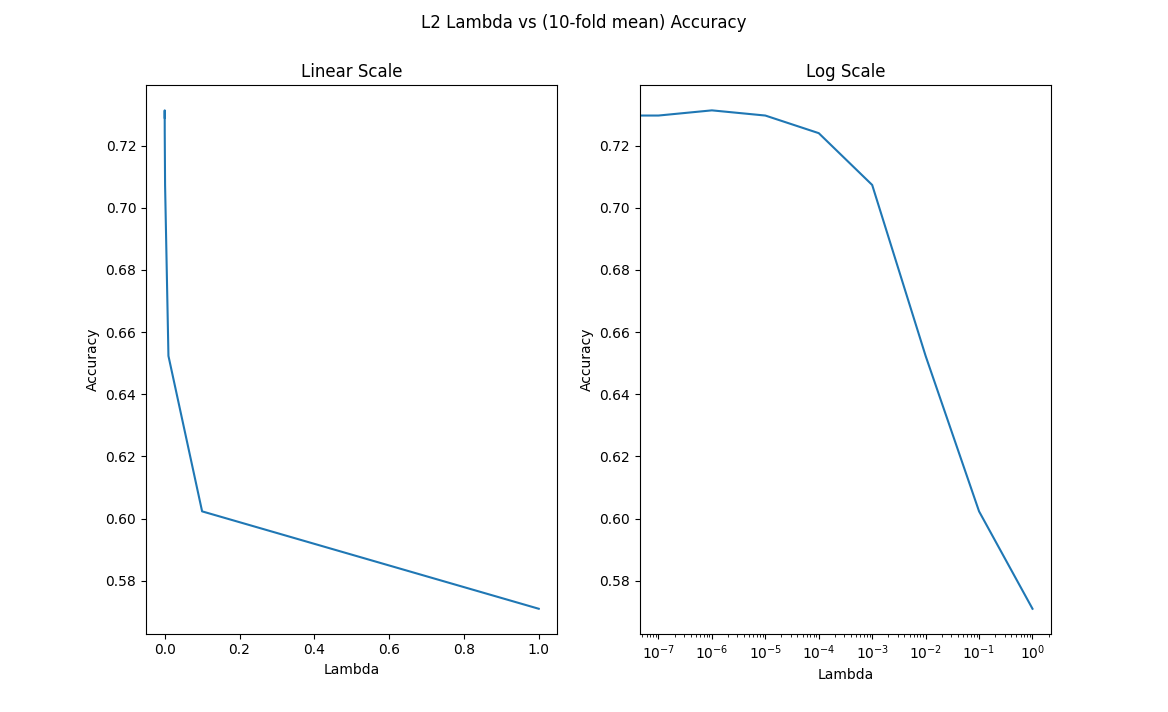
\includegraphics[scale=0.5]{lambda_graph}
\end{center}

The results seem to show that a harsher penalty (greater lambda) for a longer weight vector generally decreases the accuracy. L2 regularization serves to mitigate overfitting to a particular set, preventing the model from learning arbitrary artifacts present only in the training data. Perhaps it actually hurts the accuracy in this example because the training and test sets are from the same distribution. Since both are from the provided training set (Xtrain.csv, Ytrain.csv), perhaps the regularization is actually preventing the classifier from learning a better decision boundary for this overall training distribution.

\end{document}
